\documentclass[a4paper,10pt]{article}
\usepackage[utf8]{inputenc}
\usepackage[english]{babel}
\usepackage{indentfirst}
\usepackage{listings}
\usepackage{graphicx}
\usepackage{blindtext}
\usepackage{enumitem}
\usepackage{hyperref}
\usepackage[top=2.5cm,bottom=2.5cm,left=2.5cm,right=2.5cm]{geometry}
\pagestyle{headings}
\title{Ftp server in a datadiode}
\author{Rusu George, Boulif Ilias, Orinx Cédric}
\date{\today}

\begin{document}
\maketitle
\newpage
\tableofcontents
\newpage
\section{Concept of operations}
\subsection{Introduction to the problem}
Our client would want to prevent his research and development labs against industrial espionage. He wants to divide the company network in order to maintain every lab in an isolated environment. Thus, the critical data could not leave the company labs using the network. One problem related is assuring that all the operating systems are up to date. This could be achieved using a manual operation where an employee would manually update every node in the isolated network using a mass-storage device\footnote{A USB-key for instance.}. However, this is not the most optimized way and for sure it is not cost less and timeless for the company without mentioning that there could be dependency problems, this is prone to human errors and this could generate security vulnerabilities.

\subsection{Our solution}
In order to address this problem we are going to implement a data diode. In electronics as shown in Figure \ref{fig:diode}, a diode is a component which conduct the current in one direction. Thus the term of data diode is a set of components that only let the data to travel in an unidirectional way. An example of use case is illustrated in Figure \ref{fig:datadiode}, letting the data pass from a low risk VLAN\footnote{IEEE 802.1Q.} to a high risk VLAN but not the way around.
\begin{figure}
\centering
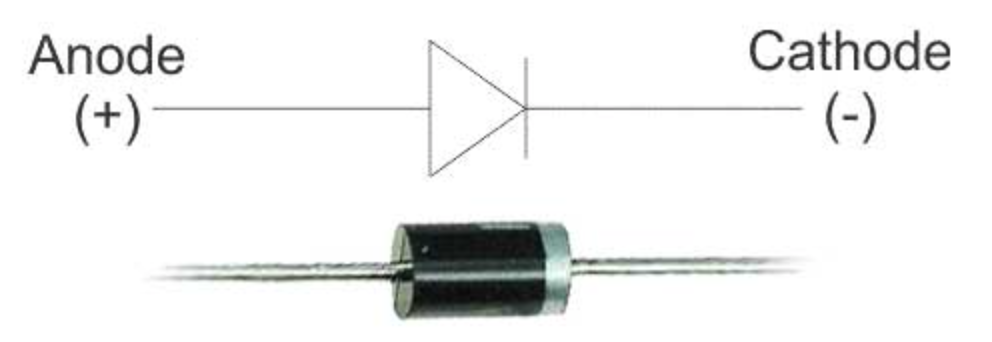
\includegraphics[scale=0.25]{images/diode.png}
\caption{A diode schema in electrionics.}
\label{fig:diode}
\end{figure}

\begin{figure}
\centering
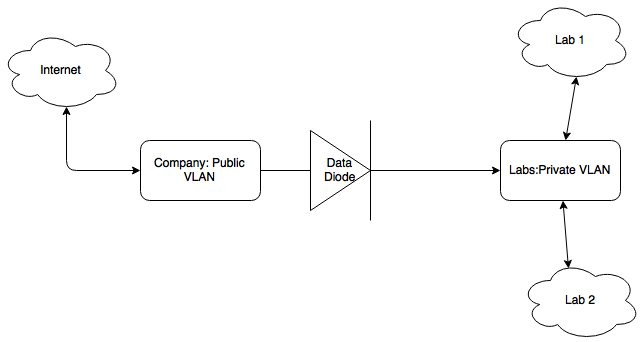
\includegraphics[scale=0.45]{images/dataDiode.png}
\caption{The schema of the usage of a data diode in a company network.}
\label{fig:datadiode}
\end{figure}

A data diode is made using a transmitter and a receiver both linked using one fiber cable. Thus, when a digital data want to be send trough, every bit will be converted\footnote{using a Digital to analog converter (DAC).} into an electrical pulse that the transmitter will convert in light pulse using a LED\footnote{Light Emitting Diode.}. Then, the output light will pass trough the fiber cable and as soon as the photons are reaching the receiver, they will be converted firstly into an electrical pulse by a photo diode and then in bits\footnote{using an analog to digital converter (ADC).}.

One major problem is the network transport protocols(layer 4 in the OSI model) that applications are using. The most used transportation protocol nowadays is TCP. However, TCP is a bi-directional protocol which means that in order to start a connection there must be at least two fiber cables (the 3 ways handshake). In contradiction, UDP does not require a handshake process in order to provide reliability, ordering, data integrity and does not set up a dedicated end-to-end connection automatically and thus does not require a bi-directional data transfer. Therefore, the use of such a protocol is recommended when dealing with applications that are not sensitive to data loss or that implements an error checking system. Hence, the UDP protocol is used within the data diode.

Furthermore, this brings multiple problems. One of the problems is how to be able to use applications that requires TCP.  TO BE CONTINUED



 
\begin{figure}
\centering
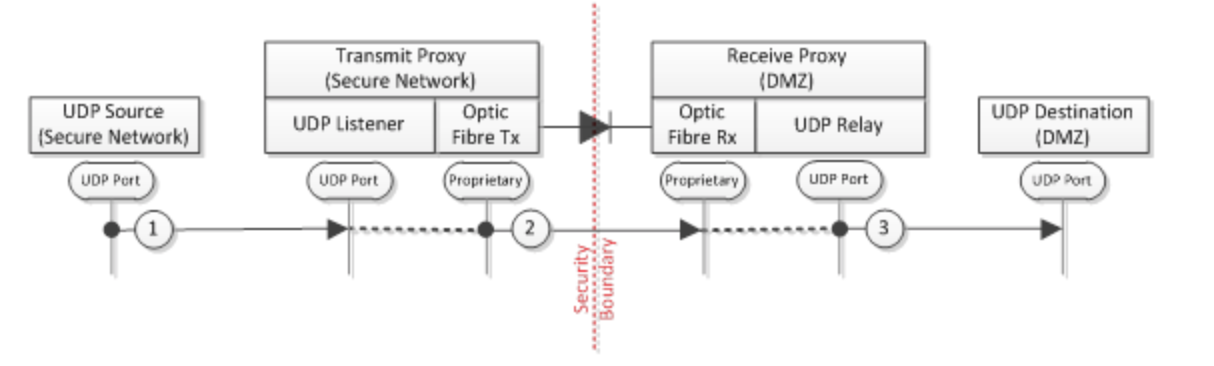
\includegraphics[scale=0.5]{images/UDPOverDD.png}
\label{fig:UDPDD}
\caption{UDP over a data diode.}
\end{figure}


\subsection{Our System description}
The data diode concept is well orchestrated combination between hardware and software. The data diode is composed by 2 server. We can consider one as a \textit{low server}, wich is connected to the Internet, and one as a \textit{high sever} wich is connected to the secure environement of the entreprise. 
The transmittion of the information will be from the low side to the high side, and blocked in the other direction (\textit{Bell-LaPadula security model}(pas sur)).

\subsubsection{Hardware}

\begin{tabular}{|p{3cm}|p{10.5cm}|}
	\hline
	\textbf{Component} & \textbf{Description}                 \\
	\hline
	2 Server "type" &    \\
	\hline
	Unidirectional optical fiber\footnote{http://www.conrad.fr/ce/fr/product/505019/Fibre-optique-unidirectionnelle-R4-M3-2M-Ftp40-Panasonic-FTP40} & This optical fiber allows communication between the low server the high server.                    \\
	\hline
	Fiber Optic Sensor & Placed on the high server
    to receive the data through the optical fiber \\
	\hline
\end{tabular}

\subsubsection{Software}

\paragraph{OS Linux} will be used for the both sever.

\paragraph{Web interface} will be used for the administration of the data diode.

\paragraph{BlindFTP}\footnote{https://www.decalage.info/fr/python/blindftp} is a simple and portable tool for transferring files over a unidirectional network link (without acknowledgment), wich is perfect for our data diaode.

\subsubsection{Objectives}
\subsection{Users} 
We will have two types of users in our system : the \textit{administrator} and the \textit{user}.\\

The \textit{administrator} is the person in charge of operating and maintaining the data diode. The only authorized person to interact with the data diode must be one (or two) \textit{administrator} designated by the company. He will have to know how it works and be able to use the administration interface\ref{UI}.\\

The \textit{user} are the employee who are on the secured network and who needs the files
transferred to maintain their computer up-to-date.\\

All users have a type, an username and a password. All these informations are
managed and stored in a database by the company.
\subsection{User Interface}\label{UI}


[idee : site web sur le transmitter, login+ mot de passe , avoir une certainte tracabilité, pouvoir umploader une fichier depuis le site et juste l'envoyer de l'autre cote. ]\\


The administration of our data diode happens through a web interface.
This web interface will be hosted on the transmitter. This will allows to get the
files from the lower network. For the user interface we have tryed to make it
easy to use. In ordre to use the interface, the first step is to log on with his
user name and password.  Once we are connected, (if we are a user??)
we are on a page that allows the file transfer from the transmitter(lower network)
to the receiver(high network), simply by a mechanism of drag and drop(or upload?).
(if we are admin??)

\textbf{TO DO : parler de la tracabilité}


\subsection{System implementation}
\subsection{General usage}
The interface will be used each time by the users from the secured network
in order to transfer a file through the data diode. By using the interface,
users can transfer the files they need by simply dragging and dropping them to
the dedicated transfer folder which is forwarded to the secure network.


\begin{thebibliography}{9}

\bibitem{nist-fips-202}
NIST,
\textit{SHA-3 Standard: Permutation-Based Hash and Extendable-Output Functions},
FEDERAL INFORMATION PROCESSING STANDARDS PUBLICATION,
2015.

\end{thebibliography}
\end{document}